\section*{DISCLAIMER} \emph{Questa sezione è un cantiere aperto. NON è definitiva in nessuna sua parte, NON nei contenuti, NON nella struttura, NON nel tono generale del discorso. Si tratta di una serie di appunti che sto prendendo e che saranno la base su cui scriverò poi la versione definitiva, li inserisco per mantenerne traccia e per avere ben chiara la direzione che sta intraprendendo il discorso.}

In questo capitolo si vuole presentare il quadro attuale della situazione attorno ai sistemi blockchain. Nuove tecnologie sono sviluppate continuamente, perciò dopo una breve panoramica sui progetti più interessanti già in stadio avanzato di sviluppo si illustreranno le sfide e gli ambiti di ricerca più ferventi, fino ad arrivare ad elencare alcune delle applicazioni che potrebbero conseguire dai risultati di tali ricerche.

\section{Innovazioni vicine}
    Al momento si assiste ad una crescita rapidissima di Bitcoin, tale da portare l'argomento al di fuori degli ambiti specialistici e farlo diventare un vero e proprio fenomeno di massa.
    \begin{figure}[ht]
        \centering
        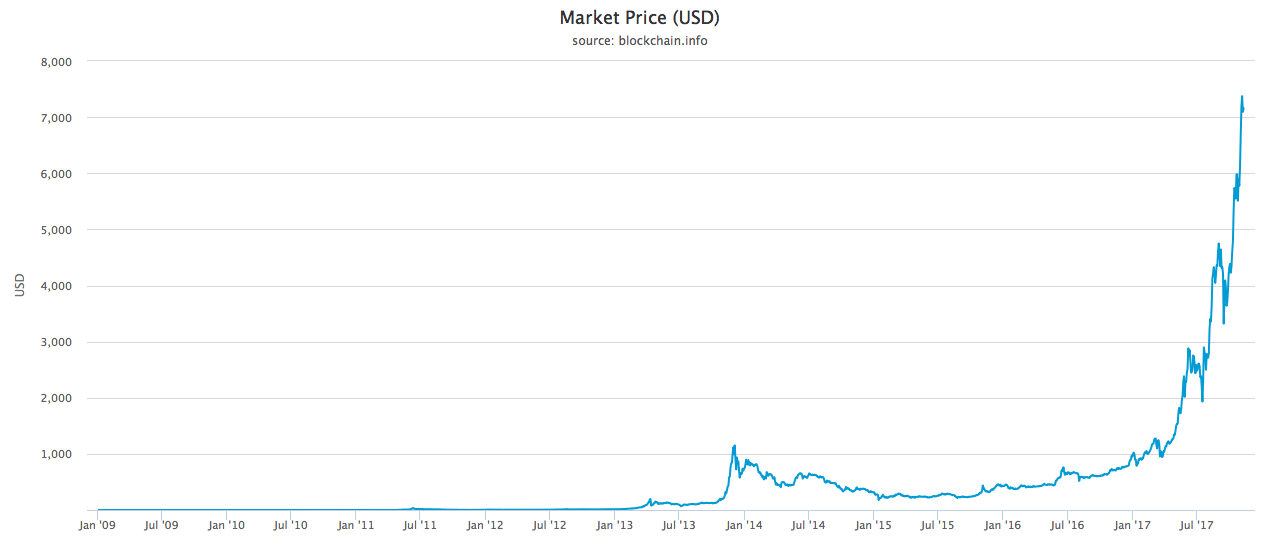
\includegraphics[width=\textwidth]{bitcoin-price.png}
        \caption{Valore di mercato di bitcoin}
        \label{fig:bitcoin_price}
    \end{figure}
    Dietro a Bitcoin si sta sviluppando un'enorme quantità di applicazioni e sperimentazioni che riguardano Blockchain, alcune delle quali hanno raggiunto ormai una certa stabilità. Molte di queste riguardano l'ambito economico e prendono il nome di \emph{criptomonete}, altre invece si basano sulla blockchain per costruire sistemi più complessi.
    \subsection{Criptomonete}
        \begin{itemize}
            \item \textbf{Ripple}: è il più famoso sistema di scambio di valuta basato su blockchain permissioned, adottato tra gli altri da MUFG, RBC, Santander, Unicredit, BBVA \url(https://ripple.com/);
            \item \textbf{Litecoin}: è una criptomoneta molto simile a Bitcoin da cui differisce per alcune caratteristiche chiave, su tutte il tempo necessario all'elaborazione di un blocco (2 minuti e mezzo contro i 10 minuti di Bitcoin) e il sistema di consenso. Litecoin infatti usa \emph{scrypt} per la sua proof-of-work, una funzione gravosa sulla memoria piuttosto che sul processore che punta a evita il predominio delle server farm con hardware dedicato che controllano le operazioni di mining di Bitcoin;
            \item \textbf{Peercoin}: è una criptomoneta alternativa che adotta un algoritmo di consenso ibrido tra proof-of-work e proof-of-stake, allo scopo di portare un'alternativa solida all'enorme consumo energetico di Bitcoin;
            \item \textbf{Monero}: fork di Bitcoin che utilizza CryptoNote, un protocollo basato sulla Ring Signature orientato a rafforzare l'anonimato nella blockchain;
            \item \textbf{ZCash e ZCoin}: come Monero si pongono l'obiettivo di garantire la privacy in un sistema Blockchain, usano algoritmi di tipo zero-knowledge sebbene con piccole differenze tra di loro \cite{zcoin_vs_zcash};
        \end{itemize}
        Un'altra applicazione interessante a livello economico è quella legata all'uso di criptomonete per il crowd-funding. Questa trova una semplice implementazione direttamente in Bitcoin attraverso l'uso di quello che si chiama \emph{assurance contract}. Si tratta di una transazione con un singolo output rappresentante l'obiettivo del finanziamento, a cui si unisce poi ciascun volontario partecipante tramite hash di tipo \emph{SIGHASH\_ALL} e \emph{SIGHASH\_ANYONECANPAY}, che permettono di modificare gli input di transazione ma non gli output (si rimanda alla documentazione ufficiale per approfondimento). La transazione può essere registrata in blockchain, e quindi essere effettiva, solo quando il valore di output è coperto da corrispondente valore in input, ovvero al raggiungimento dell'obiettivo della campagna di crowd-funding.
     
    \subsection{Non-Criptomonete}
        \begin{itemize}
            \item \textbf{Ethereum}: \emph{DA ESPANDERE E PROMUOVERE A SEZIONE ASSIEME AD HYPERLEDGER} si tratta del principale sistema basato su Blockchain dopo Bitcoin. Il suo scopo è quello di permettere la creazione di applicazioni decentralizzate, che vengono eseguite come smart contract distribuiti tra i peer che partecipano alla rete. È il primo sistema blockchain ad aver introdotto un linguaggio Turing-completo (\emph{Solidity}) e il concetto di macchina virtuale su blockchain, nel 2013. Si basa su una propria moneta virtuale che viene utilizzata per ``alimentare" le applicazioni distribuite (in ambito Ethereum si parla di \emph{gas}, abbreviazione di \emph{gasoline}). Questa si chiama \emph{Ether}, e al momento si trova saldamente al secondo posto come market cap dietro a Bitcoin;
            \item \textbf{OpenTimestamps}: servizio che mira a diventare uno standard per il timestamping via blockchain. Concatena hash crittografici dei dati di cui gli utenti richiedono il timestamping e ne registra il risultato in una transazione bitcoin, rendendolo quindi pubblico e immutabile;
            \item \textbf{Namecoin}: servizio basato su blockchain che si propone di potenziare decentralizzazione, sicurezza, resistenza alla censura, privacy e velocità di componenti alcune dell'infrastruttura di Internet come i DNS;
            \item \textbf{Everledger}: una nicchia promettente riguarda i sistemi ad-hoc con utilizzo ben preciso. Ne è un esempio Everledger, che si propone di tracciare e gestire storia e possesso di beni di lusso come i diamanti; \emph{Filament} per reti wireless sicure in IoT;
            \item \textbf{Filament}: la natura distribuita di Blockchain la rende ideale per implementazione di applicazioni IoT che richiedano un adeguato livello di sicurezza. Lavora in questo ambito Filament, startup nata recentemente, nel 2017, che si pone come obiettivo la gestione di reti wireless sicure in ambito IoT;
            \item \textbf{Blockchain a livello enterprise}: per la creazione di applicazioni aziendali basate su Blockchain è necessario appoggiarsi ad opportuni framework. Questi devono rispettare requisiti imprescindibili per l'ambito business, tra cui fornire opportuna documentazione, supporto tecnico e rendere agevoli le operazioni di testing, integrazione, controlli di sicurezza. Esempi di piattaforme simili in sviluppo sono Hyperledger, Bloq, Chain, sebbene ciascuno di questi soffra al momento di poca stabilità dovuta alla loro ancora recente nascita;
            \item \textbf{Hawk}: è un sistema di smart contract che affronta il problema della poca privacy nelle transazioni delle blockchain più diffuse. Hawk fornisce uno strumento per la generazione di un ``protocollo crittografico efficiente in cui le controparti del contratto interagiscono con la blockchain usando primitive crittografiche come gli algoritmi \emph{zero-knowledge proof}." \cite{hawk};
        \end{itemize}

\section{Sfide e ambiti di ricerca}
    \subsection{Efficienza e scalabilità}
        \begin{itemize}
            \item Algoritmi di consenso
            \item Problemi crittografici nuovi
        \end{itemize}
        Il problema della scalabilità dei sistemi blockchain è molto dipendente dall'algoritmo di consenso implementato. Quelli ad oggi adottati su larga scala sono basati su proof-of-work, che paradossalmente basa la sua sicurezza sulla sua assoluta inefficienza. Inoltre, la storia di Bitcoin mostra come sia inefficace nel mantenere equilibrata la competizione tra i miner, portando un accentramento delle capacità di gestione della rete nelle mani di server farm dedicate. Ethereum migliora questo aspetto attraverso un algoritmo simile, ma in cui ha meno vantaggi investire in hardware dedicato. Tuttavia la ricerca ad un algoritmo che permetta l'effettiva ``democratizzazione'' del mining è ancora apertissima, accompagnata da quella su problemi crittografici meno parallelizzabili su cui basare ulteriori varianti degli algoritmi proof-of-work.
        
    \subsection{Standardizzazione e interoperabilità}
        Blockchain non è ancora una tecnologia sufficientemente matura da permettere una piena ed agevole integrazione con i sistemi esistenti. Emettere degli standard adeguati aiuterà a migliorare l'integrazione dei sistemi blockchain tanto fra di loro quanto con l'infrastruttura circostante. \\
        Dal punto di vista applicativo lo sviluppo di framework come Hyperledger aiuta a creare una base solida e delle sottostrutture chiare per la progettazione di reti distribuite interoperanti, e maggiore sarà il numero di utenti che abbracceranno soluzioni di questo tipo minori saranno le differenze critiche tra sistema e sistema permettendo adattamenti più agevoli. D'altra parte, è necessario che tali piattaforme si sviluppino e allarghino la gamma di scenari modellabili venendo incontro alle necessità di gruppi di utenti sempre più grandi ed eterogenei. \\
        Dal punto di vista normativo invece si sono visti passi in avanti con la creazione nel 2016 del comitato tecnico ISO/TC 307 ``Blockchain and distributed ledger technologies", che sta sviluppando il primo standard ISO ufficiale sull'argomento.

    \subsection{Privacy}
        
        \subsubsection{Obfuscation}
            vedi pag 244 di Understanding Bitcoin
        \subsubsection{Algoritmi zero-knowledge}
            \begin{itemize}
                \item \textbf{Zero-Knowledge Password Proof} \\
                    \url{https://en.wikipedia.org/wiki/Zero-knowledge_password_proof}
                \item \textbf{Piattaforma Enigma} \\
                        \url{https://www.enigma.co/enigma_full.pdf}
                \item \textbf{zk-SNARK} \\
                    \url{https://z.cash/technology/zksnarks.html}
            \end{itemize}

\section{Cosa si potrà fare}
    \begin{itemize}
        \item Reti IoT sicure basate su Blockchain condivise
        \item Condivisione dati sensibili (cartelle cliniche?)
        \item Digital Identity
        \item Immigrazione e controlli doganali
        \item Cronotachigrafi
        \item Gestione DRM (digital rights management)
        \item Digital assets e smart properties
        \item Moneta basata su Bitcoin per transazioni efficaci tra privati
\end{itemize}
